\section{Map Node Menus}
\label{prototype:MapNodeMenus}
As I've introduced new features such as searching and node locking, I've found It frustrating to keep adding new buttons to control the features I'm working on. I wanted to add a more integrated method of control around the nodes themselves I have added node menus. Nodes can now be held right-clicked (or held down on touchscreen devices) and this menu will appear, selecting an option changes the settings of that specific node. The 'Drill Down' command acts similarly to searching for an exact node - making it easier to hide information that is not relevant to the current goal

\begin{figure}[H]
    \centering
    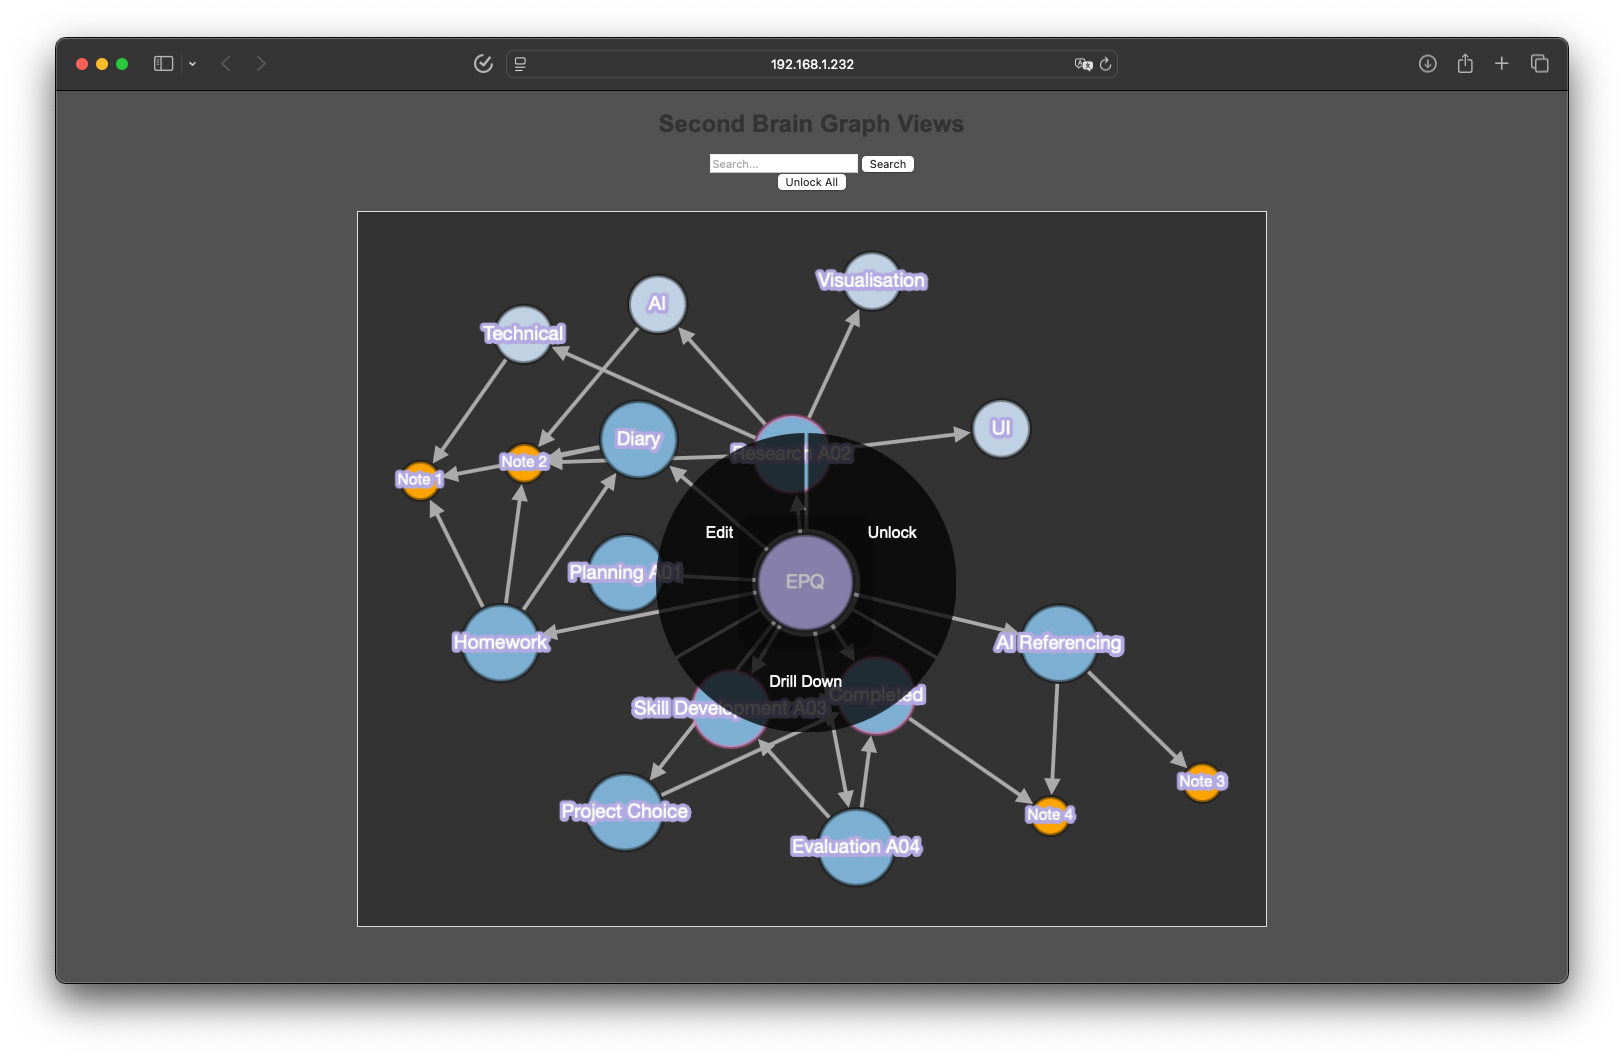
\includegraphics[width=0.8\textwidth]{Prototype/8_MapNodeMenus/media/prototype.png}
    \caption{Map Node Menus Prototype}
\end{figure}


